
%%%%%%%%%%%%%%%%%%%%%%%%%%%%%%%%%%%%%%%%%%%%%%%%%%%%%%%%%%%%%%%%%%%%%%%%%%%%%%%%%%%%%%%%%%%%%%%%%
%
% Document:      DM  SST organisation chart reporting lines
%
% Based on the DM organisation chart reporting lines by William O'Mullane
%%%%%%%%%%%%%%%%%%%%%%%%%%%%%%%%%%%%%%%%%%%%%%%%%%%%%%%%%%%%%%%%%%%%%%%%%%%%%%

\documentclass{article}

\usepackage{times,layouts}
\usepackage{tikz,hyperref,amsmath}
\usetikzlibrary{positioning,arrows,shapes,decorations.shapes,shapes.arrows}
\usetikzlibrary{backgrounds,calc}

\usepackage[paperwidth=30cm,paperheight=20.0cm,
left=-2mm,top=3mm,bottom=0mm,right=0mm,
noheadfoot,marginparwidth=0pt,includemp=false ]{geometry}


\newcommand\showpage{%
\setlayoutscale{0.5}\setlabelfont{\tiny}\printheadingsfalse\printparametersfalse
\currentpage\pagedesign}


\hypersetup{pdftitle={DM SST organisation }, pdfsubject={Diagram illustrating the reporting lines in LSST SST DM Group}, 
pdfauthor={ Leanne Guy}}


%%%%%%%%%%%%%%%%%%%%%%%%%%%%%%%%%%%%%%%%%%%%%%%%%%%%%%%%%%%%%%%%%%%%%%%%%%%%%%%%%%%%%%%%%%%%%%%%%
%
% Document:      Boxes and lines for all diagrams
%
%%%%%%%%%%%%%%%%%%%%%%%%%%%%%%%%%%%%%%%%%%%%%%%%%%%%%%%%%%%%%%%%%%%%%%%%%%%%%%

\tikzstyle{divbox}=[rectangle, rounded corners=3pt, draw=blue, top color=blue!30!white, bottom
color=white, very thick, minimum height=12mm, inner sep=3pt, text centered, text width=35mm]

\tikzstyle{arcbox}=[rectangle, rounded corners=3pt, draw=red, top color=yellow!50!white, bottom
color=white, very thick, minimum height=12mm, inner sep=2pt, text centered, text width=50mm]

\tikzstyle{psbox}=[rectangle, rounded corners=3pt, draw=red, top color=green!50!white, bottom
color=cyan, very thick, minimum height=10mm, inner sep=2pt, text centered, text width=35mm]

\tikzstyle{pobox}=[rectangle, rounded corners=3pt, draw=red, top color=blue!50!white, bottom
color=cyan, very thick, minimum height=10mm, inner sep=2pt, text centered, text width=35mm]

\tikzstyle{docbox}=[rectangle, rounded corners=3pt, draw=black, fill=cyan!50!white, 
 very thick, minimum height=12mm, inner sep=2pt,  text centered, text width=30mm]

\tikzstyle{docboxm}=[rectangle, rounded corners=3pt, draw=black, fill=red!50!white, 
 very thick, minimum height=12mm, inner sep=2pt,  text centered, text width=30mm]

\tikzstyle{docboxicd}=[rectangle, rounded corners=3pt, draw=black, fill=green!70!white, 
 very thick, minimum height=12mm, inner sep=2pt,  text centered, text width=30mm]

\tikzstyle{gbox}=[rectangle, rounded corners=3pt, draw=orange!80!black, top color=orange!30!white,
bottom color=white, very thick, minimum height=12mm, inner sep=5pt, text badly ragged, text width=40mm]

\tikzstyle{mbox}=[rectangle, rounded corners=3pt, draw=blue, top color=cyan!50!white, bottom
color=white, very thick, minimum height=8mm, inner sep=2pt, text centered, text width=30mm]

\tikzstyle{line}=[-, thick]
\tikzstyle{sline}=[-, thick, dashed, olive]
\tikzstyle{dline}=[->, thick, cyan]
\tikzstyle{tline}=[->, thick, dashed, blue]
\tikzstyle{pline}=[->, thick,  black!60!white]

\xdefinecolor{softviolet}{rgb}{0.85, 0.8, 1.0}




\begin{document}

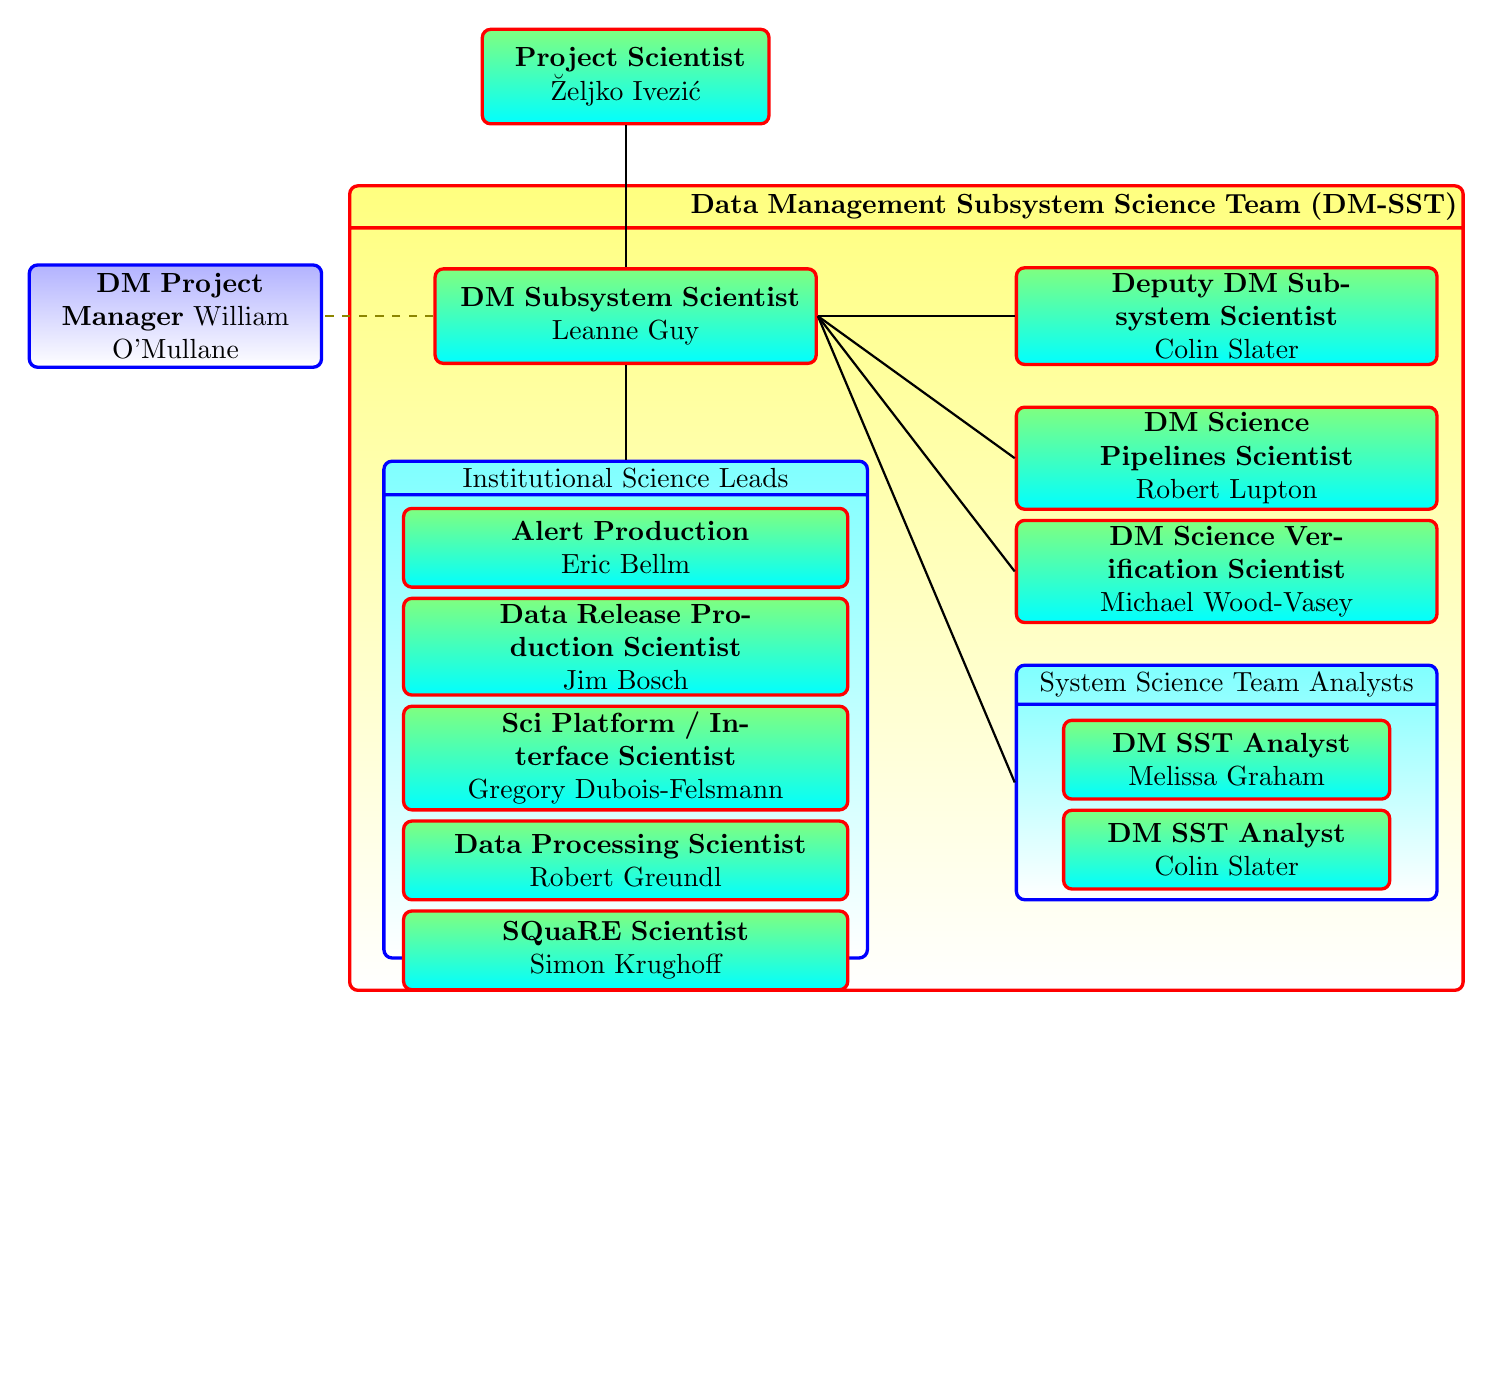
\begin{tikzpicture}[node distance=0mm]


    \node (dm) [arcbox, align=right, text width=14cm,  minimum height=10mm, rectangle split, rectangle split parts=2]
    { \hspace{0.1cm} \textbf{Data Management Subsystem Science Team (DM-SST)}
	   \nodepart{second} \vspace{95mm}
	};


   % \node (dmpm) [divbox, above=-2.5cm of dm.north] {\textbf{DM Project Manager} William O'Mullane};
    %\node (dmdpm) [divbox, left=1.5cm of dmpm] {\textbf{DM Deputy Manager} John Swinbank};
    \node (dmpsanc) [above=-1.8 of dm.north]{};
    \node (dmps) [psbox, left=1.0cm of dmpsanc, minimum height=12mm, text width=47mm] {\textbf{ DM Subsystem Scientist}\\ Leanne Guy };
    \node (ddmps) [psbox, right=2.5cm of dmps, minimum height=12mm, text width=52mm] {\textbf{ Deputy DM Subsystem Scientist}\\ Colin Slater };
    \node (ps) [psbox, above=1.8cm of dmps, minimum height=12mm] {\textbf{  Project Scientist}\\ \u{Z}eljko Ivezi\'c};
    \node (dmpm) [divbox, left=1.4cm of dmps] {\textbf{ DM Project Manager} William O'Mullane};
    
    \node (udmpm) [below=49mm of dmpm, text width=0mm]{};
    \node (udmpm1) [below=24mm of dmpm, text width=0mm]{};
    \node (udmpm2) [below=125mm of dmpm, text width=0mm]{};

% Pipelines scientist
    \node (pipesci) [psbox, below =5mm of ddmps, text width=52mm, minimum height=12mm] {\textbf{DM Science Pipelines Scientist}\\ Robert Lupton};
    
% Verification Scientist
    \node (valsci) [psbox, below=1mm of pipesci, text width=52mm, minimum height=12mm] {\textbf{DM Science Verification Scientist}\\ Michael Wood-Vasey};




% INSTLEADS
            \node (instleads) [mbox, text width=60mm, rectangle split, rectangle split parts=2,  below=12mm of dmps]
                {
               Institutional Science Leads
                \nodepart{second} \vspace{57mm}
                };
    \node (apsc) [psbox, below=6mm of instleads.north, text width=55mm] {\textbf{ Alert Production }\\ Eric Bellm };
    \node (drpsc) [psbox, below=1mm of apsc, text width=55mm] {\textbf{Data Release Production Scientist}\\ Jim Bosch};
    \node (suitsc) [psbox, below=1mm of drpsc, text width=55mm] {\textbf{Sci Platform / Interface Scientist}\\ Gregory Dubois-Felsmann};
    \node (dpsc) [psbox, below=1mm of suitsc, text width=55mm] {\textbf{ Data Processing Scientist}\\ Robert Greundl};
    \node (sqsc) [psbox, below=1mm of dpsc, text width=55mm] {\textbf{SQuaRE Scientist}\\ Simon Krughoff  };
%%%% end INSTLEADS

% SCIANALYSTS
            \node (sstanal) [mbox, text width=52mm, rectangle split, rectangle split parts=2, below=0.5cm of valsci.south ]
                {
                System Science Team Analysts
                \nodepart{second} \vspace{23mm}
                };
    \node (sstanal-mlg) [psbox, below=7mm of sstanal.north, text width=40mm] {\textbf{ DM SST Analyst }\\ Melissa Graham };
    \node (sstanal-cts) [psbox, below=1mm of sstanal-mlg, text width=40mm] {\textbf{DM SST Analyst}\\ Colin Slater};
   %%%% end SCIANALYSTS
   
%%% Legend 
%\node (leg) [lbox, below=4cm of admin, text width=35mm,  minimum height=10mm, rectangle split, rectangle split parts=2]
%    { \hspace{0.1cm} \textbf{Legend}
%           \nodepart{second} \vspace{30mm}
%        };
 %\node(snode) [psbox,below=0.7cm of leg.north, text width=30mm] {Science Role};
 %\node(pnode) [mbox,below=0.1cm of snode, text width=30mm] {Technical Role};
 %\node(mnode) [mbox,below=0.1cm of pnode, text width=30mm] {Managment/other Role};

    %\node (cm) [mbox, right=3.1cm of udmpm1.north , text width=45mm] {\textbf{Config/Release Manager }\\ Gabriele Comoretto};
    %\node (pconp) [below=5mm of cm] {};
   % \node (docu) [mbox, right=70mm of pconp , text width=45mm] {\textbf{DM Documentalist}\\ Jonathan Sick };
    %\node (pcon) [mbox, below=5mm of docu , text width=45mm] {\textbf{Project Control/Scheduler }\\ Kevin Long};
    %\node (admin) [mbox, below=5mm of pcon, text width=45mm] {\textbf{DM Admin}\\ Libby Petrick};

    %\node (pdocu) [mbox, right=5.5cm of ps, text width=45mm, minimum height=12mm] {\textbf{LSST Documentalist}\\ Robert McKercher};

    %\node (al) [below=69mm of dmpm, text width=0mm]{};
%    \dmnode[left=1mm of udmpm2.north]{suit}{SUIT}{Xiuqin Wu}{Gregory Dubois-Felsmann}{psbox} ;
%    \dmnode[base left=2mm of suit]{das}{Data Access Services}{Fritz Mueller}{Colin Slater} {psbox};
%
%    \node (drp) [mbox, text width=36mm, rectangle split, rectangle split parts=2, base left=2mm of das]
%         {Science Pipelines \strut \nodepart{second} \vspace{39mm}};
%
%         \node(drpt) [mbox,minimum height=9mm, below=8mm of {drp}.north, text width=32mm] {\parbox[height=12mm]{0pt}{}{\small \bf T/CAM}\\\strut John Swinbank \\ {\bf Deputy}\\ Yusra AlSayyad };
%         \node(drps) [psbox,minimum height=9mm, below=2pt of drpt, text width=32mm] {{\small \bf DRP Owner}\\\strut Jim Bosch};
%         \node(alerts) [psbox,minimum height=9mm, below=2pt of drps, text width=32mm] {{\small \bf Alerts Owner}\\\strut Eric Bellm};
%
%	 \dmnode[base right=2mm of suit]{square}{SQuaRE} {\strut Frossie Economou}{ Simon Krughoff }{psbox} ;
%
%    \node (infra) [mbox, text width=36mm, rectangle split, rectangle split parts=2, base right=2mm of square]
%         {Data Facility \strut \nodepart{second} \vspace{39mm}};
%
%         \node(dft) [mbox,minimum height=9mm, below=8mm of {infra}.north, text width=32mm] {\parbox[height=6mm]{0pt}{}{\small \bf T/CAM}\\\strut Margaret Gelman };
%         \node(infrapo) [pobox,minimum height=9mm, below=2pt of dft, text width=32mm] {{\small \bf Infrastructure Owner}\\\strut Michelle Butler};
%         \node(procpo) [psbox,minimum height=9mm, below=2pt of infrapo, text width=32mm] {{\small \bf Proc Systems Owner}\\\strut Robert Gruendl};
%
%	 \dmnode[base right=2mm of infra]{lhn}{LHN \& Base Site}{Jeff Kantor}{Michelle Butler}{pobox} ;

 %% GROUPS ..

   %  \node (dmsg) [psbox, below=0.5cm of dmps, minimum height=12mm] {\textbf{DM Subsystem Science Team}};
    % \node (dmlt) [mbox, left=1cm of man.west , text width=25mm] {\textbf{DMLT }};

   % \draw[line] (dmps.south) --  (dmsg.north);
   \draw[line] (dmps.north) --  (ps.south);
    \draw[sline] (dmps.west) --  (dmpm.east);
   \draw[line] (ddmps.west) --  (dmps.east);
   
    \draw[line] (dmps.east) --  (pipesci.west);
     \draw[line] (dmps.east) --  (valsci.west);
     \draw[line] (dmps.south) --  (instleads.north);
    \draw[line] (dmps.east) --  (sstanal.west);
      
 %   \draw[line] (dmlt.east) --  (man.west);

   %\draw[line] (dmpm.north) -- ++(0,0.8) -| (pm.south);
  %s \draw[line] (dmdpm.east) --  (dmpm.west);

%dm lines second number is the proportional turning point of the line
  % \draw[line] (alerts.north) -- ++(0,0.3) -| (dmpm.south);
%   \draw[line] (drp.north) -- ++(0,0.3) -| (dmpm.south);
%   \draw[line] (das.north) -- ++(0,0.3) -| (dmpm.south);
%   \draw[line] (suit.north) -- ++(0,0.3) -| (dmpm.south);
%   \draw[line] (square.north) -- ++(0,0.3) -| (dmpm.south);
%   \draw[line] (infra.north) -- ++(0,0.3) -| (dmpm.south);
%   \draw[line] (lhn.north) -- ++(0,0.3) -| (dmpm.south);

%   \draw[line] (instleads.east) to (udmpm.north);
%   %\draw[line] (cm.west) -| (udmpm1.north);
%   \draw[line] (pcon.west) -| (udmpm1.north);	
%   \draw[line] (docu.west) -| (udmpm.north);
%   \draw[line] (admin.west) -| (udmpm.north);
%science
%   \draw[sline] (ps.west) to (pm.east);
%   \draw[sline] (dmps.west) to (dmpm.east);
%
%   \draw[sline] (docu.north) -|  (pdocu.south);

\end{tikzpicture}
\end{document}